\chapter[Results analysis]{\centering \begin{normalsize} \begin{Huge}
		Results analysis
		\end{Huge} \end{normalsize}}
\label{ch:mdp_results}

In this chapter, the effects on the GNSS positioning from smartphones introduced by the application of the MDP algorithm are discussed. In particular the performance of the algorithm, in terms of multipath detection and mitigation, by varying its configuration parameters are exposed. For this purpose both static and kinematic datasets are analysed. 

\section{Processing strategy}

The datasets analysed for the evaluation of the performance of the proposed algorithm are the case studies 3 and 4 reported in chapter \ref{ch:quality_analisys}. The selected case studies are used to test the main features of the proposed architecture. They are both processed using the LIGE base station, developed for this work. They  require the use of our Android app installed on a device and the modified RTKLIB version for data processing. Although the proposed architecture has been designed for real-time applications, in order to evaluate the performance of the MDP algorithm, several post processing elaborations were computed all having the same input data, hence  under  the same contextual conditions.

%TIZIANO: non ricordo se c'è un altra sezione della tesi in cui i valori di soglia e i criteri con cui è stato creato l'MDP sono dettagliati meglio.

The MDP algorithm present several input parameters to tune the computation phase. First of all, in the detection step one out of three criterion must be selected. Moreover, the strategy for the MDP threshold computation must be chosen between the static and the adaptive one. The value chosen as static threshold remains constant for the entire computation. For the adaptive threshold value, the number of previous epochs should be set. The MDP threshold will depend then on a  statistical analysis computed on the previous MDP values following the equation \ref{eq:mdpthres_dyn}.  Finally the SNR threshold must be set.  

The values to be associated with the various parameters to achieve optimal results may depend on various factors (e.g. environmental conditions and hardware characteristics of the receiver) and are still object of research. For the two case studies, some PPK processing were performed considering different combinations of those parameters, as later explained. 

Concerning the rest of the processing options used in RTKLIB for PPK positioning, the Ionosphere and Troposhere models used are the Klobuchar and Saastamoinen respectively. Only the broadcast ephemeris were considered and an elevation mask of \ang{15} is also set. The solution type selected is "forward" for both  case studies.

%TIZIANO: spiegare il motivo delle scelte di processing indicate al precedente paragrafo.
\section{Experimental Results}
This section presents the results of the processing carried out with the application of the MDP algorithm. Preliminary considerations on the MDP value are made for both case studies considered. From these considerations, the different values to associate with the various configuration parameters of the MDP algorithm are then chosen. Finally, the results obtained from the different processing are presented and discussed.

The static test with induced multipath (i.e. test 4 in Chapter \ref{ch:quality_analisys}) is analysed first.  This dataset is particularly interesting as we can analyse the behaviour of the algorithm both in the absence and presence of multipath. After that a kinematic dataset (i.e. test 3 in Chapter \ref{ch:quality_analisys}) is analysed and discussed. Finally general considerations on the performance of the MDP algorithm for smartphone's GNSS positioning are exposed.

\subsection{Static test}

As shown in chapter \ref{ch:quality_analisys}, the static dataset selected for testing the MDP algorithm refers to a static acquisition performed the 10\textsuperscript{th} March 2022 using two GNSS receivers in parallel: the Xiaomi Mi8 and the Ublox ZED F9P. Between 9:45 and 10:00 UTC a metal plate was placed behind the two receivers inducing the multipath effect. In this time interval the MDP variable is expected to have some outliers indicating the presence of multipath.
Before proceeding in the analysis of our results, the MDP trend is presented for both the receiver used, with the purpose of understanding the MDP performance in detecting multipath errors for smartphone receivers with respect to a classic GNSS receiver.

Figure \ref{FIG:test4mdp_mdpxiaomiublox} shows the MDP values detected by the Xiaomi Mi8 and the Ublox ZED F9P.

\begin{figure}[H] 
	\centering
    \subfigure[]{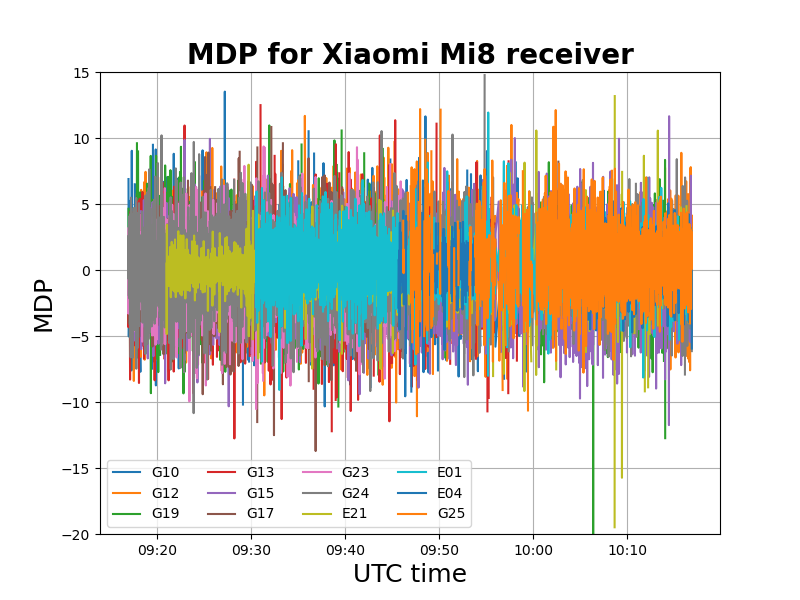
\includegraphics[width=0.48\textwidth]{fig/test4mpd/mdp_xiaomi_test4.png}} 
    \subfigure[]{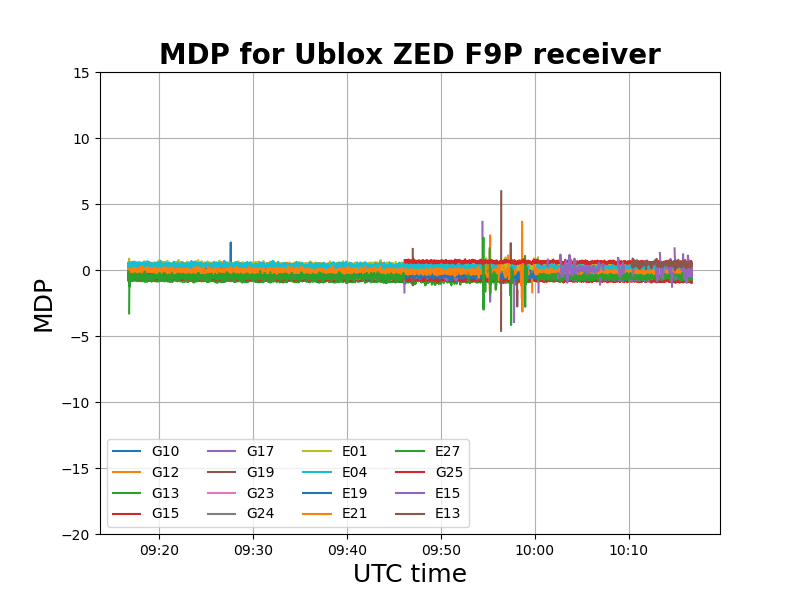
\includegraphics[width=0.48\textwidth]{fig/test4mpd/mdp_ublox_test4.png}} 
    \caption{MDP values for Xiaomi Mi8 receiver (a) and for Ublox ZED F9P receiver (b) for the static dataset}
   % \label{fig:foobar}
	\label{FIG:test4mdp_mdpxiaomiublox} 
\end{figure}

As explained in chapter \ref{FIG:dev_rtk_arch}, the MDP variable is representative of the multipath effect and residual errors due to external noise (see eq. \ref{eq:mdpvariable}). Figure \ref{FIG:test4mdp_mdpxiaomiublox} shows that the MDP variable for the Ublox ZED F9P receiver has some peaks between the 9:45 and 10:00 UTC, i.e. when the multipath effect was induced. The MDP variable than can then be considered a reasonable multipath indicator for this kind of receivers.
For the Xiaomi Mi8 receiver the MDP variable presents a  noisy trend with higher values in modulus. Differently from the Ublox ZED F9P, the Xiaomi Mi8 MDP trend has more diffuse peaks and not particularly concentrated between  9:45 and 10:00 UTC. Nevertheless, a couple of peaks can be noted for the Xiaomi Mi8 in that interval. The noisier trend of the  Xiaomi Mi8 MDP variable with respect to the Ublox ZED F9P ones, can be justified by  higher values of the external noise caused by the poor quality of the smartphone's antenna. This makes MDP variable less effective in multipath identification for smartphones receivers.  

For evaluating the performance of the MDP algorithm for the smartphone receiver, several processing were computed changing the configuration parameters. Data were processed using all the three criterion proposed for multipath detection. For every criterion, both static and adaptive MDP threshold were used as specified below.
\begin{itemize}
\item Concerning the static threshold 6 values were selected on the basis of the MDP trend (Fig. \ref{FIG:test4mdp_mdpxiaomiublox}a). The chosen value of the MDP static threshold are: 2.5, 3.0, 3.5, 4.0, 4.5 and 5 m.
\item For the adaptive threshold, 6 different windows (number of epochs) are selected: 10, 20, 30, 40, 50 and 60. The window size times the acquisition rate determine  an initialization time in which the algorithm can't be applied. Considering that all smartphones have an acquisition rate of 1 Hz, an initialisation time no longer than 1 minute (i.e. 60  epochs) was considered in the experiments.
\item  Finally, considering the SNR trend for the Xiaomi Mi8 receiver (figure \ref{FIG:test4_snr}a) 4 values of the SNR threshold were considered: 20, 25, 30 and 35 DB-Hz. 
\end{itemize}
 Combining all these option values, we considered 108 different experimental tests. Hereafter the most interesting results are reported.  

First of all, the processing results obtained for the criterion 1, i.e. considering only the MDP variable and not the SNR are exposed. In this set of tests it's possible to observe the impact on the solution of different MDP threshold values. The solutions obtained for the static mdp threshold values, compared with the solution without the MDP algorithm application, are shown in Fig.  \ref{FIG:test4mdp_crit1mdpstaticall}.

\begin{figure}[H] 
	\centering
    \subfigure[]{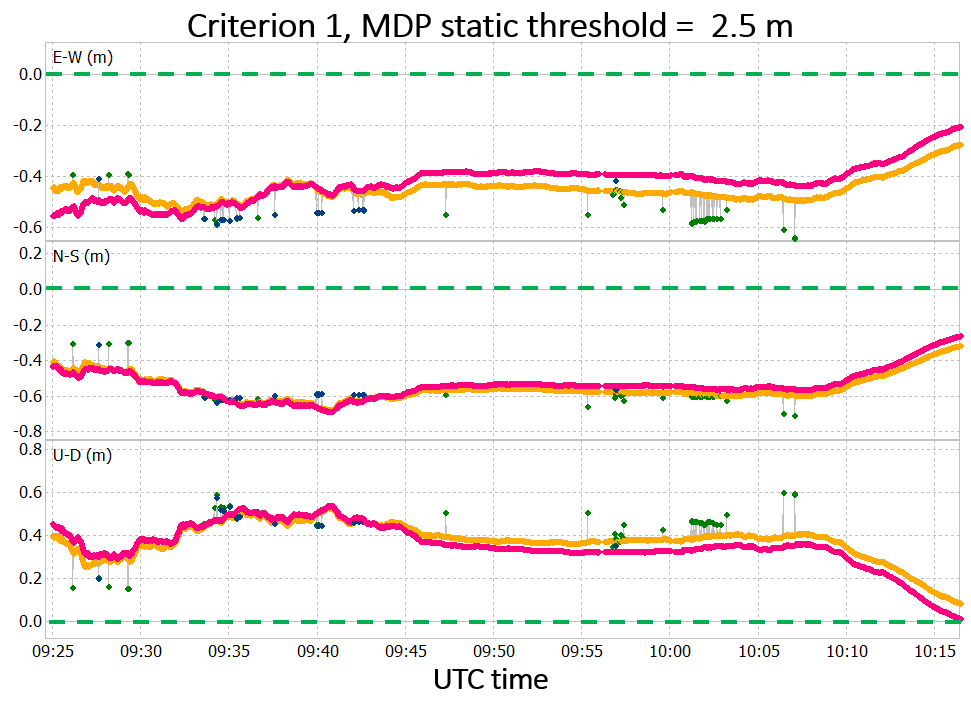
\includegraphics[width=0.48\textwidth]{fig/test4mpd/crit1_mdp_static_25.png}} 
    \subfigure[]{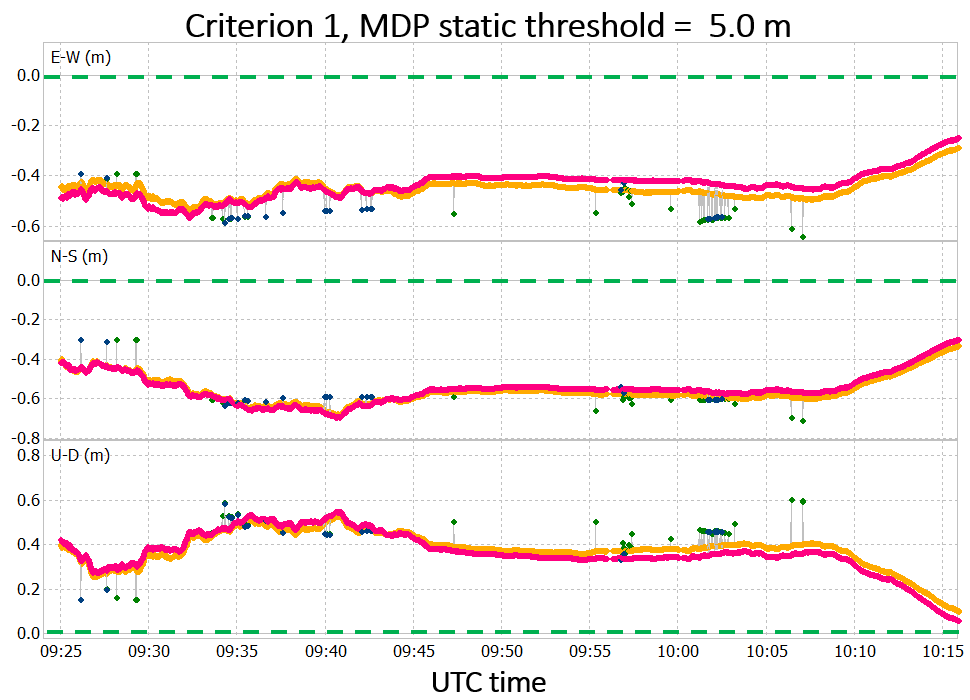
\includegraphics[width=0.48\textwidth]{fig/test4mpd/crit1_mdp_static_50.png}} 
    \caption{Results obtained after the mdp algorithm application using the criterion 1 and static mdp threshold equal to 2.5 m (a) and equal to 5.0 m (b)}
    %\label{fig:foobar}
	\label{FIG:test4mdp_crit1mdpstaticall} 
\end{figure}

In figure \ref{FIG:test4mdp_crit1mdpstaticall} the solution obtained after the MDP algorithm application are depicted in pink and blue for float and fixed solution respectively, while the solution obtained without the application of MDP algorithm is depicted in yellow and green for float and fixed solution respectively. In the figure are also highlighted the precise coordinates of the point with the dashed green line. As exposed in chapter \ref{ch:quality_analisys} this dataset presents a convergence time of about 5 minutes which is not considered for the results analysis. 

The solution, after the application of the MDP algorithm, has slight improvements in terms of accuracy, specially in the case of MDP threshold = 2.5. In this case, in fact, the solution's RMS pass from 0.450 m to 0.427 m for the East component, from 0.554 m to 0.538 m for the North component and from 0.387 to 0.370 for the Height component. The planimetric RMS of the reference solution, i.e. the one without the application of the MDP algorithm is equal to 1.428 m, while the one obtained considering the MDP static threshold equal to 2.5 m, is equal to 1.374 m. So considering the planimetric accuracy, an improvement of 5 cm is obtained.
Over all the threshold values considered for this criterion, this is the best result reached. The worst result obtained instead is the one having an MDP threshold value of 5.0 m. The difference between the two cases in terms of RMS is 2 cm for the East component, 1 cm for the North component and 1 cm for the Altitude, resulting in a RMS planimetric difference of about 2 cm. No difference in term of precision were found as the two solutions present the same STD values. 
Having noticed an improvement in the solution in terms of accuracy as the threshold value decreased, two further cases were tested with threshold values of 2.0 m and 1.5 m. However, no significant improvement has been noted with respect to the value of 2.5 m, which is therefore considered to be the best choice if a static MDP threshold is considered. 

As additional experiment, the dataset has  been  processed considering the adaptive MDP threshold. The behaviour of the adaptive threshold by varying the window size  is depicted in figure \ref{FIG:test4mdp_adaptivethr}. For instance, Fig. \ref{FIG:test4mdp_adaptivethr} is referred to the satellite G12, but the same considerations can be deduced for the other satellites.  

\begin{figure}[H] 
	\centering
    \subfigure[]{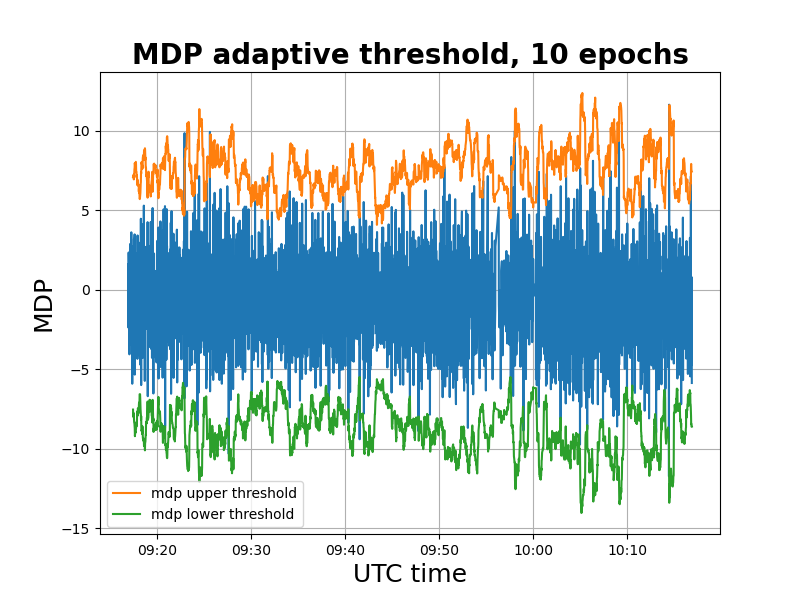
\includegraphics[width=0.48\textwidth]{fig/test4mpd/adaptive_thres_10.png}} 
    \subfigure[]{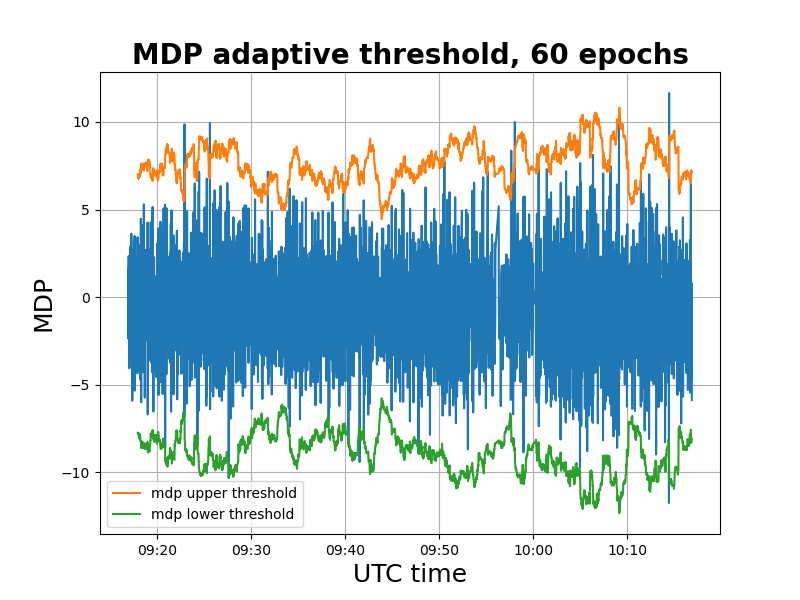
\includegraphics[width=0.48\textwidth]{fig/test4mpd/adaptive_thres_60.png}} 
    \caption{Adaptive mdp threshold trend by varying the number of previuos epochs: 10 epochs (a), 60 epochs (b)}
    %\label{fig:foobar}
	\label{FIG:test4mdp_adaptivethr} 
\end{figure}

Figure \ref{FIG:test4mdp_adaptivethr} only shows  the two extreme cases considered for the adaptive threshold computation, i.e. 10 and 60 previous epochs. It turns out  that the trend for the adaptive threshold computed over 60 previous epochs is smoother than the one computed over 10 previous epochs. Nevertheless, the capability of recognising outliers for the two cases is very similar. The positioning results by varying the number of previous epochs are pretty the same, and no appreciable differences in terms of RMS and STD can be noted in the obtained results. For this reason, hereafter all the considerations on the adaptive threshold are referred to the intermediate case among all tests, i.e. a window with 30 epochs.  

The positioning results concerning the processing executed with the criterion 1 and the adaptive MDP threshold compared with the solution without the MDP algorithm application are reported in Fig. \ref{FIG:test4mdp_crit1mdpadaptive}.

\begin{figure}[H] 
	\centering
    {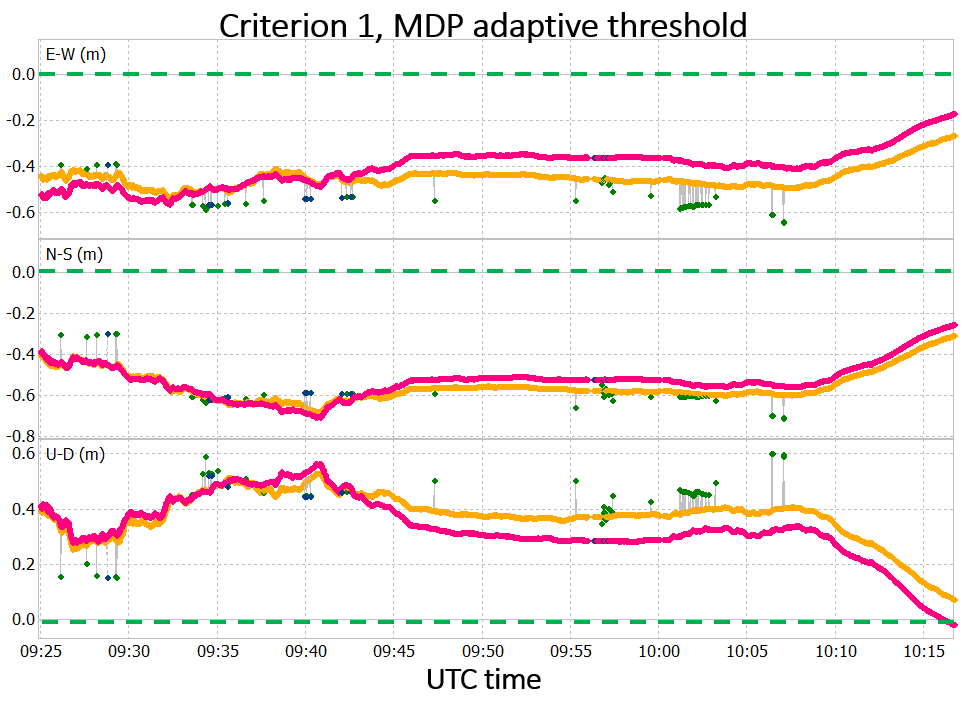
\includegraphics[width=0.50\textwidth]{fig/test4mpd/crit1_mdp_adaptive.png}}
    \caption{Results obtained after the MDP algorithm application using the criterion 1 and adaptive MDP threshold}
    %\label{fig:foobar}
	\label{FIG:test4mdp_crit1mdpadaptive} 
\end{figure}

Again, in Fig. \ref{FIG:test4mdp_crit1mdpadaptive}, the solution obtained with the application of the MDP algorithm is the one in pink and blue whereas  the solution obtained without its application is the one in yellow and green; the precise coordinates of the point are represented by the dashed green line.
In this case  improvements are present in the solution accuracy not only with respect to the case without the MDP algorithm application, but also with respect to the case with the static MDP threshold equal to 2.5 m. The difference in terms of RMS for the three cases is reported in Table \ref{tab:mdp_c1_rms}.

\begin{table}[H]
	\centering
	\begin{tabular}{|c|c|c|c|c|}
	\hline
	\textbf{Processing} & \textbf{RMS E [m]} & \textbf{RMS N [m]} &
	\textbf{RMS H [m]} &
	\textbf{RMS 2D [m]}\\
    \hline
	No MDP & 0.450 & 0.554& 0.387&1.428\\ 
    \hline
	MDP, crit 1 static thres. & 0.427 & 0.538& 0.370&1.374\\
    \hline
    MDP, crit 1 adaptive thres. & 0.410 & 0.530 & 0.353&1.339\\  
    \hline
	\end{tabular} 
	\caption{Comparison between RMS obtained after MDP application, criterion 1 }
	\label{tab:mdp_c1_rms}
\end{table}

From table \ref{tab:mdp_c1_rms}, it's possible to see that the RMS improvement obtained with the using of the adaptive threshold is of 17 mm for East and Height components and 8 mm for the North component resulting in a RMS planimetric improvement of 34 mm. This behaviour can be explained by the fact that the adaptive threshold is more selective than the static threshold in the identification of data potentially affected by multipath. Dealing with very noisy GNSS observables such as those produced by smartphones, the usage of a static MDP threshold may lead to consider as outlier in the MDP trend data that are not affected by multipath. Reducing the weights of those data still leads to some benefits in terms of positioning accuracy, but those benefits are lower with respect to the ones obtained if only multipath affected observables (i.e. outliers in the MDP trend) will be assigned a reduced weight. Concerning the precision of the solution obtained to appreciable differences are noted in the STD of the solutions, so it can be state that the MDP algorithm does not lead to improvement in positioning precision.

Concerning these processing, it's also interesting to analyse the obtained results during the period of the induced multipath only, i.e. from 9:45 to 10:00 UTC. From figures \ref{FIG:test4mdp_crit1mdpstaticall} and \ref{FIG:test4mdp_crit1mdpadaptive} it can be seen that the best improvements are obtained in that time interval, while for the rest of the period the solutions with and without the application of the MDP algorithm are quite similar. The solution obtained for both adaptive and static threshold in that time interval are depicted in Fig. \ref{FIG:test4mdp_crit1mpind}.

\begin{figure}[H] 
	\centering
    \subfigure[]{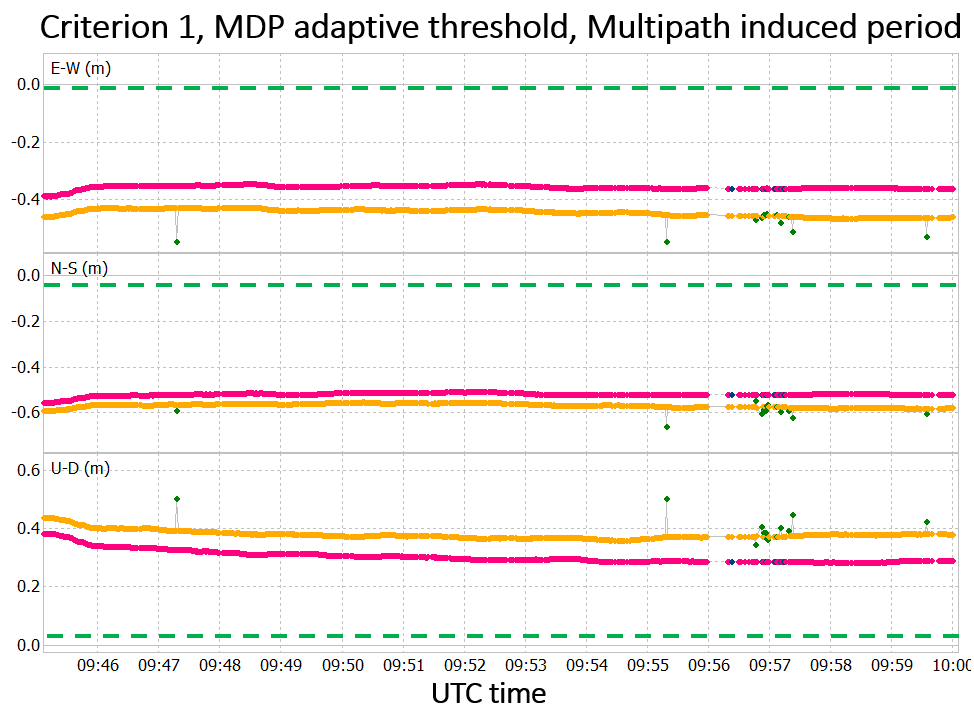
\includegraphics[width=0.48\textwidth]{fig/test4mpd/crit1_mdp_adaptive-mpind.png}} 
    \subfigure[]{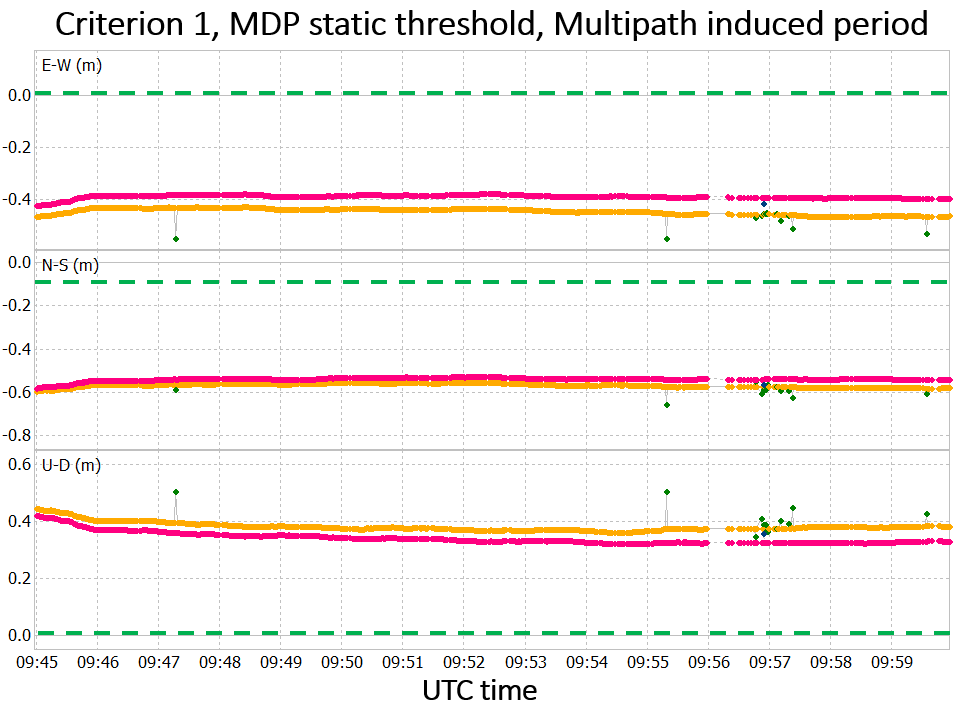
\includegraphics[width=0.48\textwidth]{fig/test4mpd/crit1_mdp_static-mpind.png}} 
    \caption{Results obtained after the MDP algorithm application using the criterion 1 and adaptive MDP threshold (a) and static MDP threshold (b) referred to the multipath induced interval}
   % \label{fig:foobar}
	\label{FIG:test4mdp_crit1mpind} 
\end{figure}

 The color criteria used for Fig. \ref{FIG:test4mdp_crit1mpind} is the same adopted for Fig. \ref{FIG:test4mdp_crit1mdpstaticall} and Fig. \ref{FIG:test4mdp_crit1mdpadaptive}.

It is possible to observe from figure \ref{FIG:test4mdp_crit1mpind} that  the solution obtained with the MDP algorithm presents an unstable set of fixed solutions. However, fixed solutions obtained without the MDP algorithm turned out to be  often false solutions. Indeed, their RMS is in the order of tens of centimeters, while, for fixed solution, the expected RMS should be in the order of few centimeters. In this sense, an unstable set of results  that is still consistent with the rest of the obtained positions seems to be preferable to false fixed solutions. Therefore, the MDP heuristics seems to increase the robustness of the positioning process in the selected test battery.

The differences in terms of RMS for the adaptive threshold case and static  one, are reported in table \ref{tab:mdp_crit1_mpind_table}.
\begin{table}[H]
	\centering
	\begin{tabular}{|c|c|c|c|c|}
	\hline
	\textbf{Processing} & \textbf{RMS E [m]} & \textbf{RMS N [m]} &
	\textbf{RMS H [m]}&
	\textbf{RMS 2D [m]}\\
    \hline
	No MDP & 0.444 & 0.567& 0.384&1.441\\  
    \hline
	 MDP, crit 1 static thres.& 0.387 & 0.5393& 0.344&1.328\\ \hline
	 MDP, crit 1 adaptive thres.& 0.356 & 0.519& 0.309&1.259\\ \hline
	\end{tabular} 
	\caption{Comparison between RMS obtained after MDP application, criterion 1, during multipath induced interval}
	\label{tab:mdp_crit1_mpind_table}
\end{table}

Similarly to the whole test period, in this time interval the solution accuracy increases in particular when the adaptive threshold is considered. In this case an improvement of about 9 cm, 5 cm and 8 cm is obtained for East, North and Height components respectively with respect to the ``No MDP" case, resulting in a planimetric RMS improvement of 18 cm. Considering that the multipath error, was manually induced in this time interval, MDP algorithm seems to be  effective in mitigating this type of errors.

As explained in chapter \ref{ch:service_devel}, the criterion 1 that the MDP algorithm implements for the detection phase, relies only on the MDP variable; The SNR value is not considered in this phase. Criterion 2 and 3 instead exploit also SNR for this purpose. Hereafter the role that SNR plays in the MDP algorithm for multipath detection is discussed.

In criterion 2, the observable is considered affected by multipath if its SNR value is lower than its threshold and at the same time, the MDP value in modulus is higher than the current MDP threshold. Considering the static MDP threshold, coherently to the results obtained for the criterion 1, the major improvements are obtained for MDP threshold equal to 2.5 m, so the impact of the SNR value is discussed only for this situation. Figure \ref{FIG:test4mdp_crit2mdpstatic} shows the results obtained for the application of the criterion 2 considering a SNR threshold of 20 and 35 DB-Hz.

\begin{figure}[H] 
	\centering
    \subfigure[]{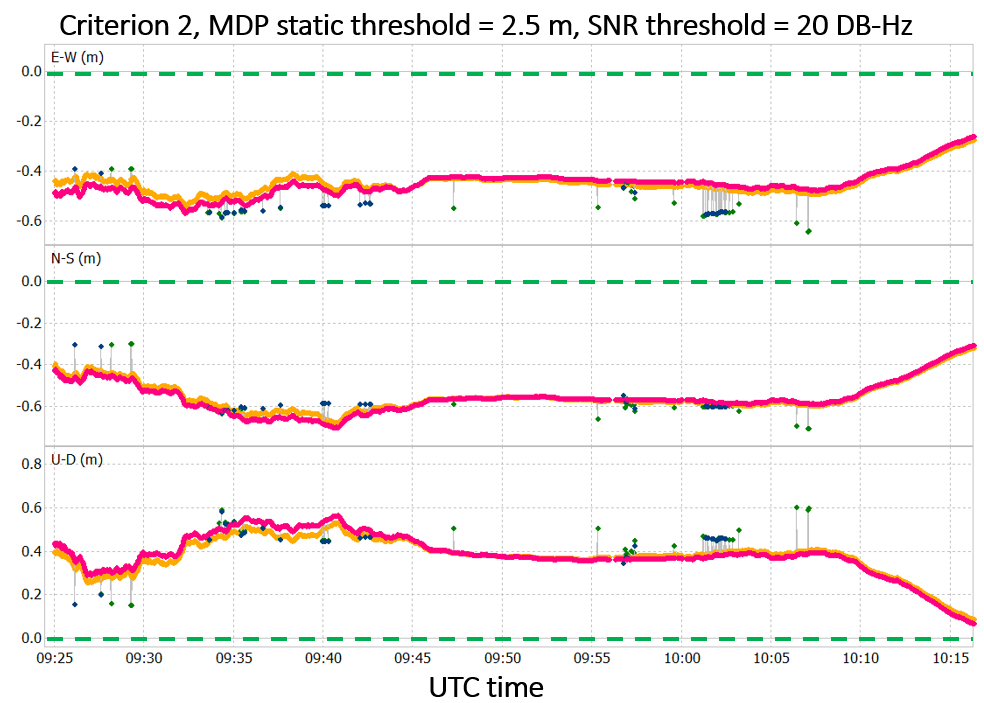
\includegraphics[width=0.48\textwidth]{fig/test4mpd/crit2_mdp_static_25_snr20.png}} 
    \subfigure[]{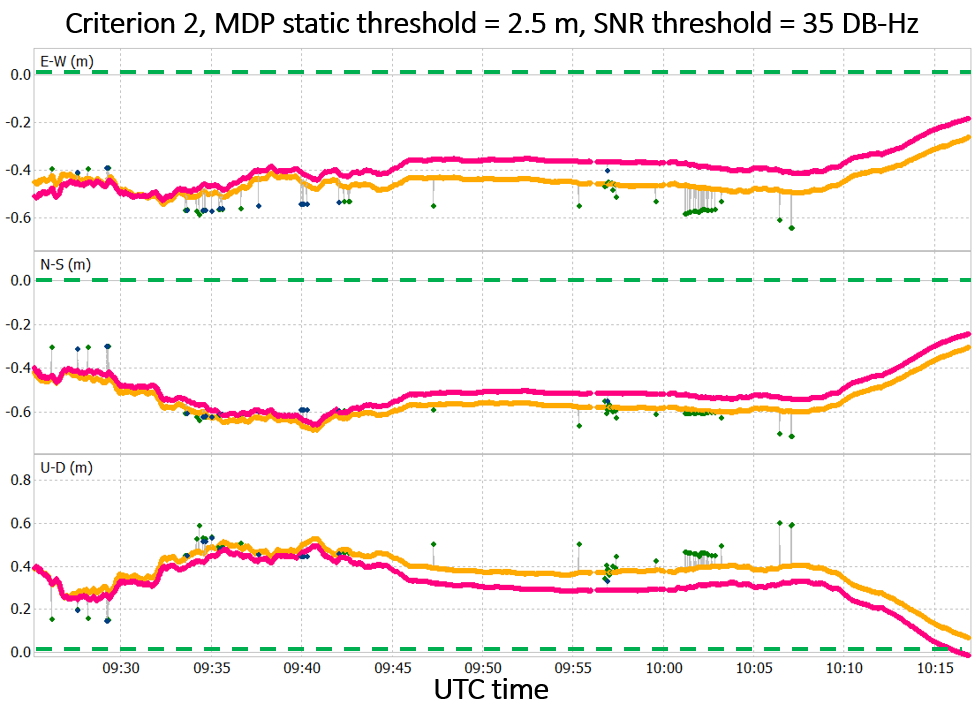
\includegraphics[width=0.48\textwidth]{fig/test4mpd/crit2_mdp_static_25_snr35.png}} 
    \caption{Results obtained after the mdp algorithm application using the criterion 2, static mdp threshold equal to 2.5 m and SNR threshold equal to 20 DB-Hz (a) and equal to 35 DB-Hz (b)}
    %\label{fig:foobar}
	\label{FIG:test4mdp_crit2mdpstatic} 
\end{figure}
In Fig. \ref{FIG:test4mdp_crit2mdpstatic} the solution obtained after the application of the MDP algorithm are depicted in pink and
blue for float and fixed solution respectively, while the solution obtained without the application of MDP algorithm is depicted in yellow and green for float and fixed solution respectively. The statistics in terms of RMS referred to the processing shown in Fig. \ref{FIG:test4mdp_crit2mdpstatic} are reported in table \ref{tab:mdp_crit2_mdp_table}.

\begin{table}[H]
	\centering
	\begin{tabular}{|p{4.5cm}|c|c|c|c|}
	\hline
	\textbf{Processing} & \textbf{RMS E [m]} & \textbf{RMS N [m]} &
	\textbf{RMS H [m]}&\textbf{RMS 2D [m]}\\
    \hline
	No MDP & 0.450 & 0.554& 0.387&1.441\\  
    \hline
	 MDP, crit 2, MDP thr = 2.5 m, SNR thr = 20 DB-Hz.& 0.448 & 0.551& 0.384&1.424\\ \hline
	 MDP, crit 2, MDP thr = 2.5 m, SNR thr = 35 DB-Hz.& 0.397 & 0.509& 0.333&1.250\\ \hline
	\end{tabular} 
	\caption{Comparison between RMS obtained after MDP application, criterion 1}
	\label{tab:mdp_crit2_mdp_table}
\end{table}

In the case of SNR threshold set to 20 DB-Hz, very low improvements can be noted in term of accuracy with respect to the solution without the MDP algorithm. This means that very few observations have the condition on MDP (i.e. $|MDP| \geq$ \textit{MDP threshold}) and on SNR (i.e. $SNR \leq$ \textit{SNR threshold}) verified at the same time and consequently very few data are annihilated by the heuristics. Considering then the results obtained with the application of criterion 1 for the same MDP threshold value (see table \ref{tab:mdp_c1_rms}), it can be stated that, for the criterion 2, the introduction of a very low SNR threshold worsens the performance of the algorithm in improving the accuracy of the solution. Also, no significant improvements in terms of solution robustness can be observed in this case. 
In fact, in figure \ref{tab:mdp_crit1_mpind_table}a about the same number of false fixed solutions are computed resp. in the test with the algorithm applied (blue points) and  without (green points).
Considering the case having SNR threshold equal to 35 DB-Hz instead some improvements in terms of accuracy can be observed. In particular an improvement of about 5 cm is obtained for East and North and Height components with respect to the solution without the MDP algorithm application. Also considering the results obtained with the application of criterion 1 for the same MDP threshold value (see table \ref{tab:mdp_c1_rms}), some accuracy improvements can be observed. In particular an RMS improvement of about 3 cm for East and North components and about 5 cm for the Height components. Furthermore if a SNR threshold equal to 35 DB-Hz is considered the number of false fixed solution is reduced with respect to the ``No MDP" case. This means that the solution robustness is increased.
Some tests were carried out for the criterion 2 also using the adaptive MDP threshold. In these cases no significant differences were obtained with respect to the results for the criterion 1. Indeed, as previously noted, the MDP adaptive threshold, differently from the static one, only selects few outliers in the MDP trend. The SNR threshold instead selects many data, especially if its value is set to 35 DB-Hz. In this case almost all the data observed satisfy the SNR condition (cfr figure \ref{FIG:test4_snr}a). Considering that for criterion 2 the MDP and SNR condition must be verified at the same time, it's reasonable to think that the discarded  data in this case are the same of those selected via 
criterion 1 where the SNR is not checked for the detection part of the algorithm.

Summarizing it's possible to state that, considering the criterion 2, the usage of the SNR values for the detection phase of the MDP algorithm takes advantages for the mitigation performance of the algorithm itself, if a static MDP threshold is considered. Those benefits regards the position accuracy and robustness and they are more evident for increasing values for the SNR threshold. No differences are introduced by the usage of SNR in the detection part if the MDP adaptive threshold is selected. No appreciable differences can be observed, for all the processing executed for this criterion, in terms of STD. It can be said so that the MDP algorithm doesn't influence the positioning precision.

Lastly the criterion 3 is considered for the processing referred to this dataset. In this criterion the observable is considered affected by multipath if the SNR of the observable is lower than the current threshold or the MDP value is higher in modulus than the current MDP threshold. In other words we reduce the weights of each piece of data selected by the condition on the SNR together and of those selected via the  condition on the MDP. Considering the static MDP threshold, coherently to the results obtained for the others two criteria, the major improvements are obtained for MDP threshold equal to 2.5 m, so the impact of the SNR value is discussed only for this situation. In criterion 3, improvements on the solution are observed only for SNR values lower than 30 DB-Hz. Figure \ref{FIG:test4mdp_crit3mdpstatic} shows the results obtained for SNR threshold equal to 25 (best results obtained for this criterion) and 35 DB-Hz (worst results obtained obtained for this criterion).

\begin{figure}[H] 
	\centering
    \subfigure[]{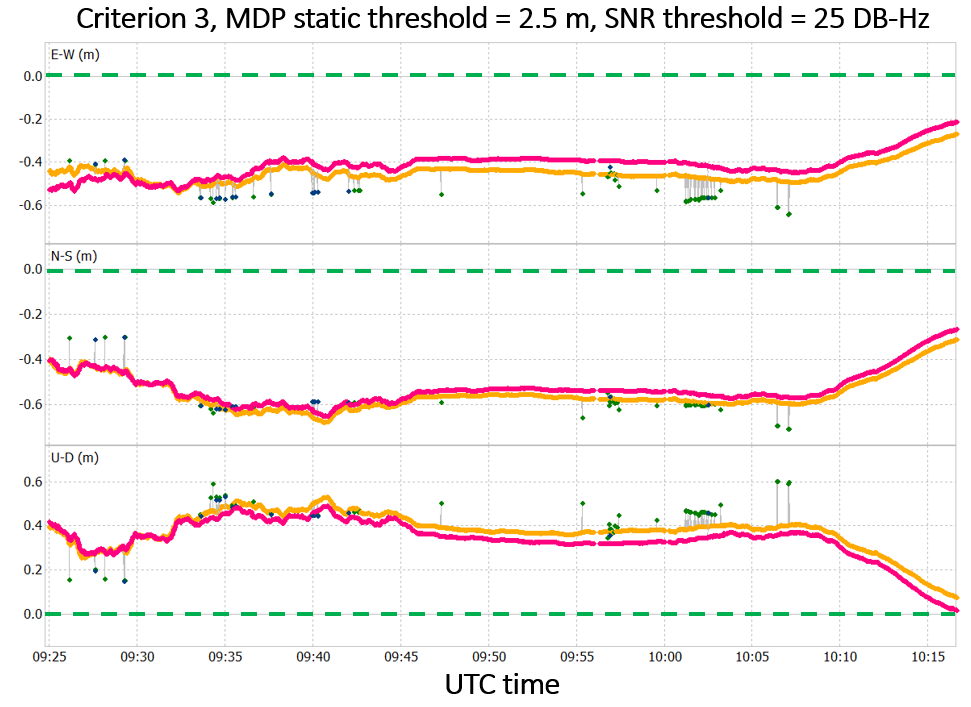
\includegraphics[width=0.48\textwidth]{fig/test4mpd/crit3_mdp_static_25_snr25.png}} 
    \subfigure[]{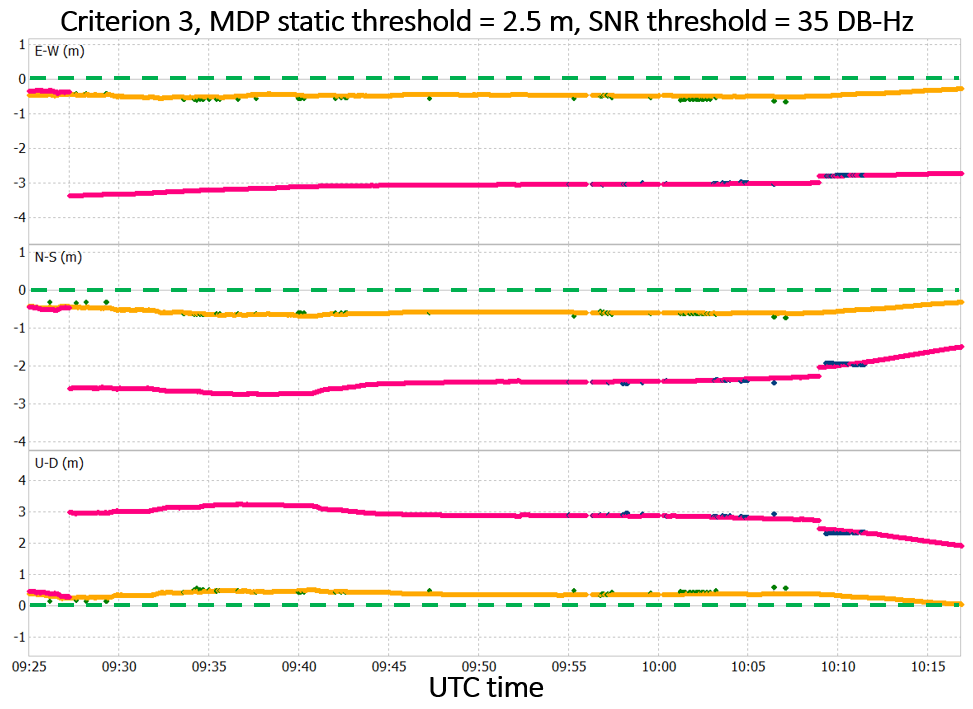
\includegraphics[width=0.48\textwidth]{fig/test4mpd/crit3_mdp_static_25_snr35.png}} 
    \caption{Results obtained after the MDP algorithm application using the criterion 3, static MDP threshold equal to 2.5 m and SNR threshold equal to 25 DB-Hz (a) and equal to 35 DB-Hz (b)}
    %\label{fig:foobar}
	\label{FIG:test4mdp_crit3mdpstatic} 
\end{figure}

The color criteria for Fig. \ref{FIG:test4mdp_crit3mdpstatic} follows the one used by the other figures reported in this paragraph. Furthermore the part a and b of the figure present different scales on the y axis, otherwise the difference between the solution obtained with the MDP algorithm (pink and blue points) couldn't be noticed for the case having SNR threshold equal to 25 DB-Hz.
The statistics in terms of RMS referred to the processing shown in Fig. \ref{FIG:test4mdp_crit3mdpstatic} are reported in Table \ref{tab:mdp_crit3_mdp_table}.

\begin{table}[H]
	\centering
	\begin{tabular}{|p{4.5cm}|c|c|c|c|}
	\hline
	\textbf{Processing} & \textbf{RMS E [m]} & \textbf{RMS N [m]} &
	\textbf{RMS H [m]}&
	\textbf{RMS 2D [m]}\\
    \hline
	No MDP & 0.450 & 0.554& 0.387&1.441\\  
    \hline
	 MDP, crit 3, MDP thr = 2.5 m, SNR thr = 25 DB-Hz.& 0.416 & 0.529& 0.354&1.346\\ \hline
	 MDP, crit 3, MDP thr = 2.5 m, SNR thr = 35 DB-Hz.& 2.974 & 2.346& 2.822&5.455\\ \hline
	\end{tabular} 
	\caption{RMS obtained for criterion 3, static MDP threshold}
	\label{tab:mdp_crit3_mdp_table}
\end{table}

From Table \ref{tab:mdp_crit3_mdp_table} it can be observed that some small improvements in terms of RMS are obtained if the SNR threshold value is set to 25 DB-Hz. Also the number of false fix solution is reduced especially between the 9:45 and the 10:00 UTC, when the multipath effect is introduced. Considering the SNR threshold value equal to 35 DB-Hz instead, the RMS of the solution is definitely degraded with respect to the one of the ``No MDP" solution (yellow and green points in figure \ref{FIG:test4mdp_crit3mdpstatic}). 

Taking into account the SNR trend of the observable, shown in Fig. \ref{FIG:test4_snr}a, and the logic of the criterion 3, it is possible to state that almost all the observables are underweighted. Even when the multipath is not present (i.e. before the 9:45 and after the 10:00 UTC) in fact the smartphone observable are very noisy as shown by their SNR values which are below 35 DB-Hz. From the obtained results, it is possible to state that underweighting all data with the proposed methodology (i.e. using equation \ref{eq:rtklib_mdp_variance}) even when they are not clearly affected by multipath, not only does not provide any benefit but  decreases the accuracy of the solution. 

Similar considerations can be also retrieved if the adaptive MDP threshold is adopted in the criterion 3.  Fig. \ref{FIG:test4mdp_crit3mdpadaptive} and Table \ref{tab:mdp_crit3_mdp_table_adaptive} shows the results obtained for SNR threshold equal to 25 (best results obtained for this criterion) and 35 DB-Hz (worst results obtained obtained for this criterion).

\begin{figure}[H] 
	\centering
    \subfigure[]{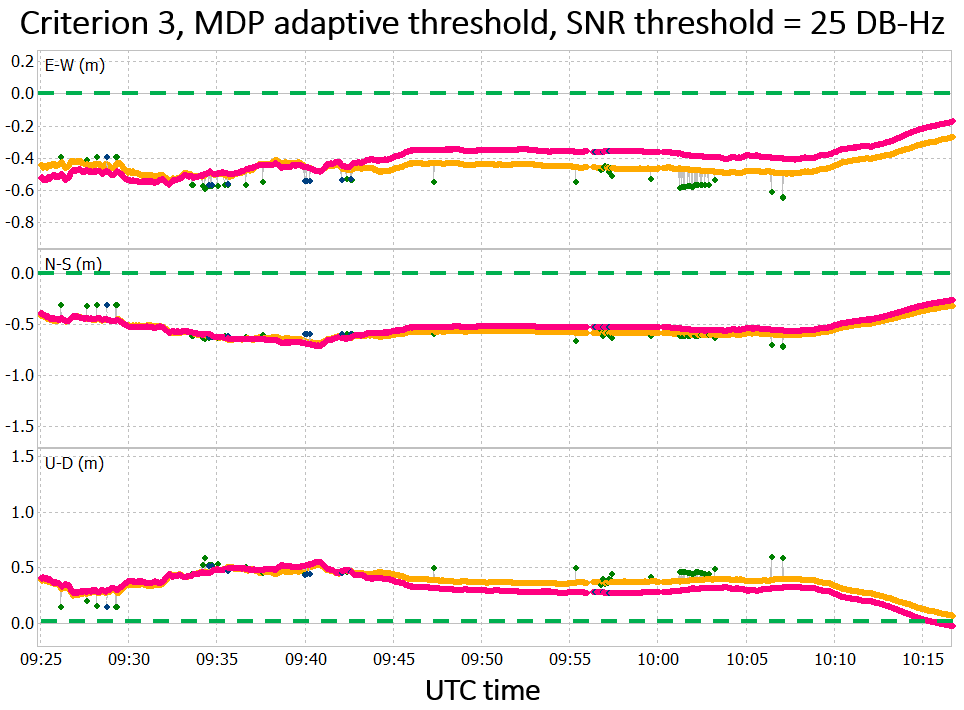
\includegraphics[width=0.48\textwidth]{fig/test4mpd/crit3_mdp_adaptive_snr25.png}} 
    \subfigure[]{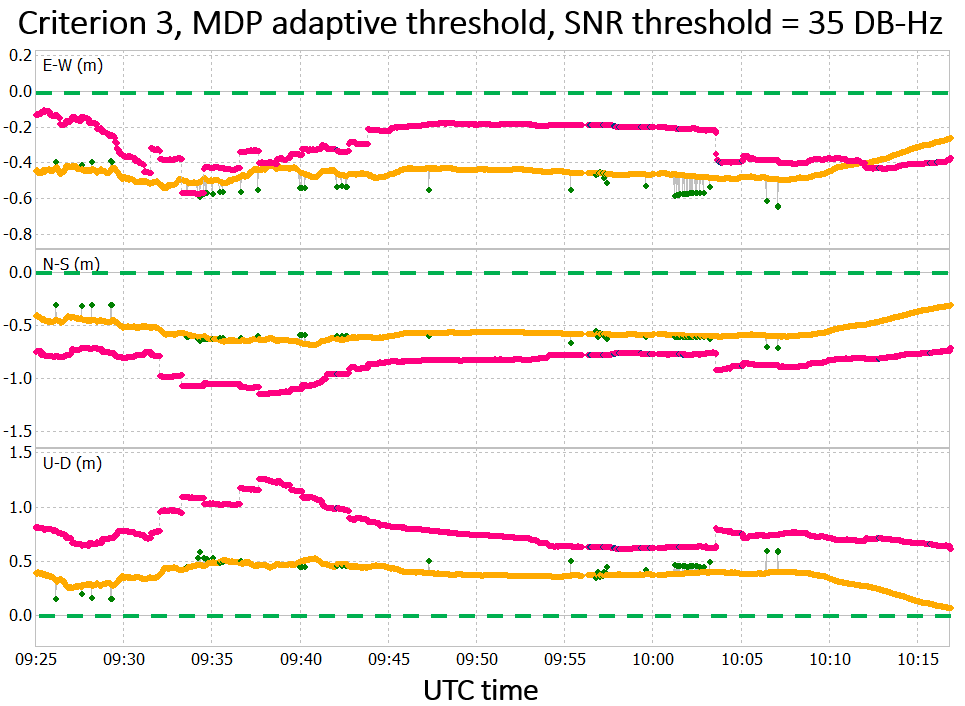
\includegraphics[width=0.48\textwidth]{fig/test4mpd/crit3_mdp_adaptive_snr35.png}} 
    \caption{Results obtained after the MDP algorithm application using the criterion 3, adaptive MDP threshold and SNR threshold equal to 25 DB-Hz (a) and equal to 35 DB-Hz (b)}
    %\label{fig:foobar}
	\label{FIG:test4mdp_crit3mdpadaptive} 
\end{figure}

\begin{table}[H]
	\centering
	\begin{tabular}{|p{4.5cm}|c|c|c|c|}
	\hline
	\textbf{Processing} & \textbf{RMS E [m]} & \textbf{RMS N [m]} &
	\textbf{RMS H [m]}&
	\textbf{RMS 2D [m]}\\
    \hline
	No MDP & 0.450 & 0.554& 0.387&1.441\\  
    \hline
	 MDP, crit 3, adaptive MDP thr, SNR thr = 25 DB-Hz.& 0.407 & 0.528& 0.353&1.333\\ \hline
	 MDP, crit 3, adaptive MDP thr, SNR thr = 35 DB-Hz.& 0.318 & 0.862&0.819& 1.837\\ \hline
	\end{tabular} 
	\caption{RMS obtained for criterion 3, adaptive MDP threshold}
	\label{tab:mdp_crit3_mdp_table_adaptive}
\end{table}
In this case, considering an SNR threshold value equal to 25 DB-Hz (Fig. \ref{FIG:test4mdp_crit3mdpadaptive}a), some millimeter-level differences are observed whit respect to the results obtained for the adaptive threshold cases of criterion 1 and 2. Considering higher SNR threshold values, e.g. SNR threshold equal to 35 DB-Hz (figure \ref{FIG:test4mdp_crit3mdpadaptive}b), similarly to the results obtained for the static threshold, the accuracy of the solution is degraded. The RMS actually presents an improved value, with respect to the ``NO MDP" case, if the East component is considered, but definitely coarser values if North and Height component are considered. 

Summarizing the results obtained for criterion 3, it is possible to state that the usage of the SNR values for the detection phase of the MDP algorithm produces benefits in the solution only if very low SNR threshold (i.e. 20 or 25 DB-Hz) are considered. However increasing the SNR threshold, almost the totality of the observables are considered affected by multipath and consequently underweighted by the MDP algorithm. This leads to a coarser solution with respect to the one obtained without the MDP algorithm application.

\subsection{Kinematic test}

As shown in Chapter \ref{ch:quality_analisys} the kinematic dataset selected for testing the MDP algorithm, refers to a kinematic pedestrian acquisition performed the 9\textsuperscript{th} of December 2021 in Genoa in Piazzale San Francesco d'Assisi using two GNSS receivers in parallel: the Xiaomi Mi8 and the Stonex S500. The acquisition was performed walking between four corners of known coordinates. At the beginning and at the end, 2 minutes of static acquisitions were performed at one of four corners considered.

As for the static case study, the MDP trend is presented for both receivers, with the purpose of understanding the MDP performance of detecting multipath for smartphone receivers with respect to more traditional GNSS receivers.

\begin{figure}[H] 
	\centering
    \subfigure[]{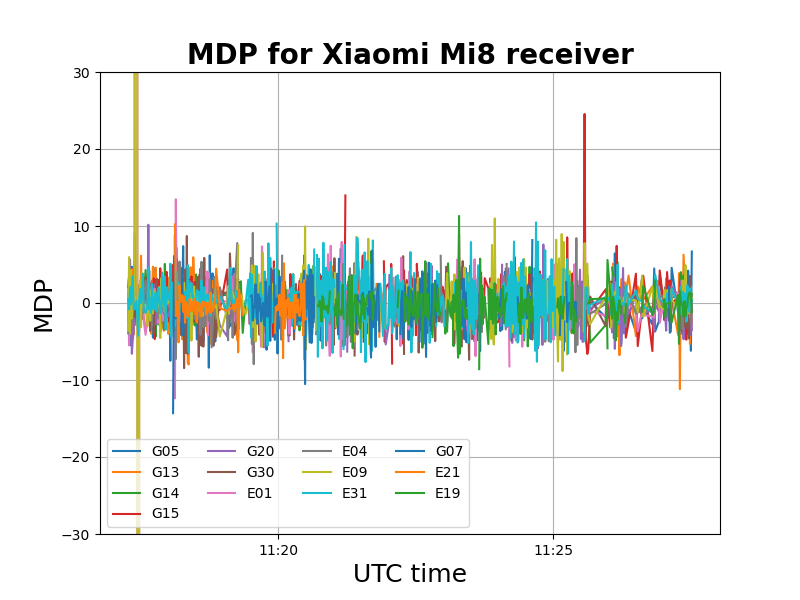
\includegraphics[width=0.48\textwidth]{fig/test3mdp/test3_mdp_xiaomi.png}} 
    \subfigure[]{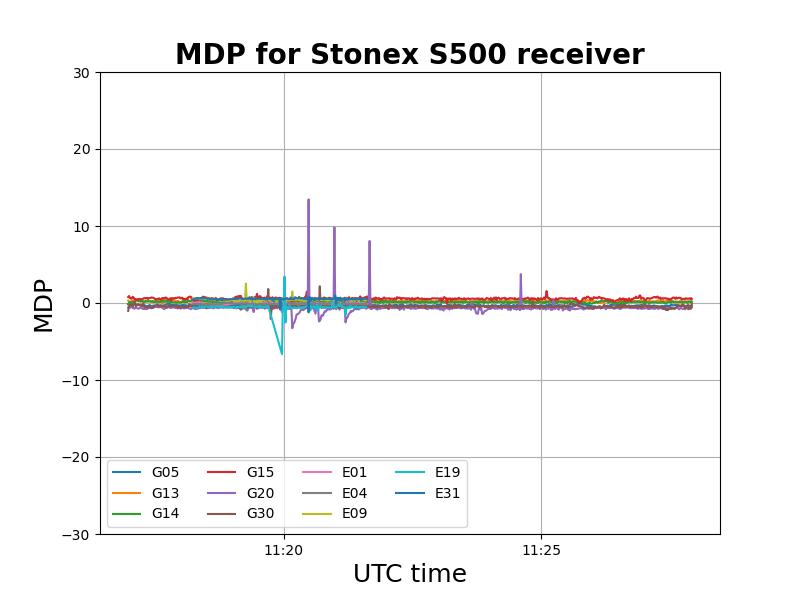
\includegraphics[width=0.48\textwidth]{fig/test3mdp/test3_mdp_stonex.png}} 
    \caption{MDP values for Xiaomi Mi8 receiver (a) and for Ublox ZED F9P receiver (b) for a kinematic dataset}
    %\label{fig:foobar}
	\label{FIG:test3mdp_mdpxiaomistonex} 
\end{figure}

Similarly to what observed for the static case study, the MDP variable for the smartphone receiver (Fig. \ref{FIG:test3mdp_mdpxiaomistonex}a) is noisier with respect to the one of a classic GNSS receiver. This confirms that, for smartphones receivers the MDP variable is less effective in multipath recognition with respect to a classical GNSS receiver. In fact, mainly due 
 to the poor quality of smartphone's antenna, the external noise component of the MDP variable is not negligible with respect to the multipath effect which is therefore not clearly identified by this method.
 
For evaluating the performance of the MDP algorithm for the smartphone receiver, several tests were performed by changing the configuration parameters. Similarly to the static case study, data were processed using all the three criterion proposed for multipath detection. For every criterion, both static and adaptive MDP threshold were used. Concerning the static threshold, 6 values were selected on the basis of MDP trend (Fig. \ref{FIG:test3mdp_mdpxiaomistonex}a). The chosen value MDP static threshold are: 2.5, 3.0, 3.5, 4.0, 4.5 and 5 m. For the adaptive threshold, due to the consideration retrieved for the static case study only 30 previous epochs were considered for the threshold computation. Finally considering the SNR trend for the Xiaomi Mi8 receiver (Fig. \ref{FIG:test3_snr}a) 4 values of the SNR threshold were considered: 20, 25, 30 and 35 DB-Hz. Combining all these option values, 63 different processing were obtained. Hereafter the obtained results are reported.

The processing results related to the criterion 1 are exposed first. Concerning all the static MDP threshold values tested, a similar behaviour has been found for all the solution obtained. The best results for this case, were obtained considering the MDP threshold equal to 2.5 m.
Fig. \ref{FIG:test3mdp_crit1mdpstatic} shows the solutions obtained for this processing, separating the initial static part by the kinematic part of the dataset.

\begin{figure}[H] 
	\centering
    \subfigure[]{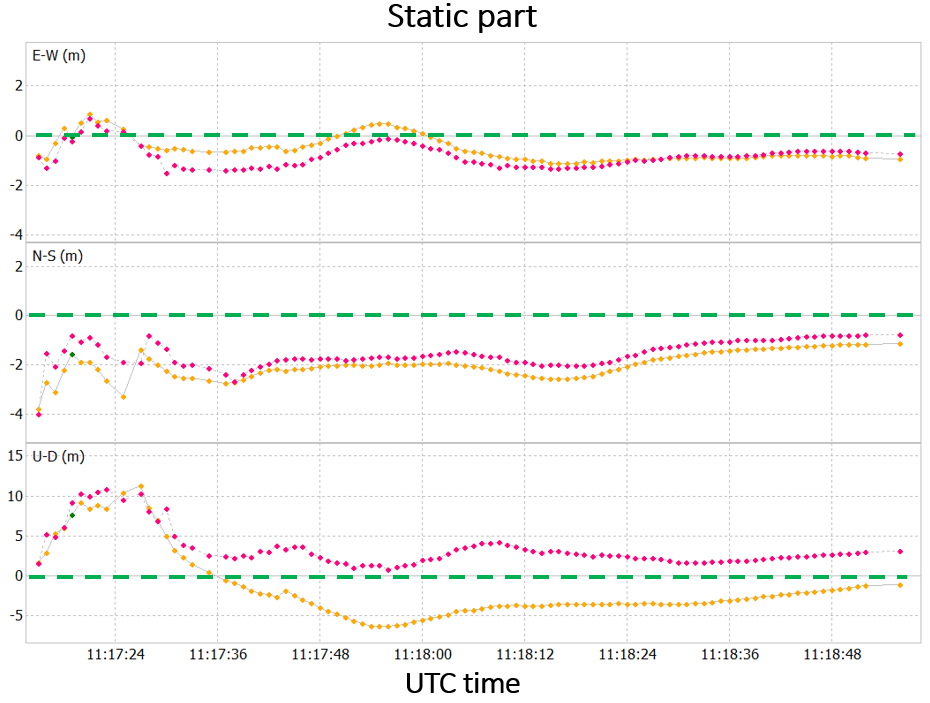
\includegraphics[width=0.48\textwidth]{fig/test3mdp/test3_crit1_m25_static.png}} 
    \subfigure[]{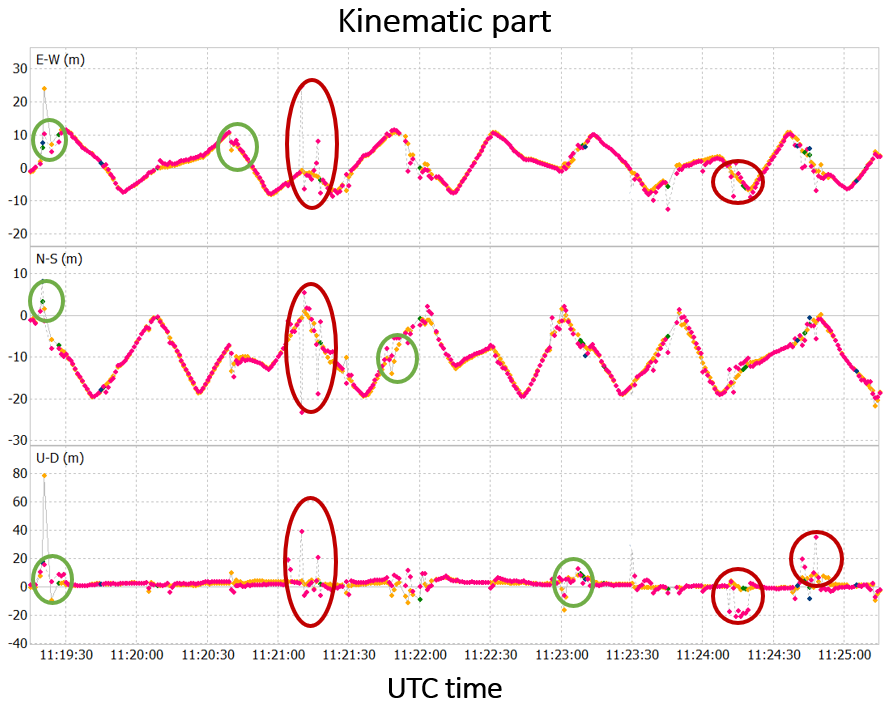
\includegraphics[width=0.48\textwidth]{fig/test3mdp/test3_crit1_m25_kin.png}} 
    \caption{Results obtained after the MDP algorithm application using the criterion 1 and static MDP threshold equal to 2.5 m for static part (a) and kinematic part (b)}
    \label{fig:foobar}
	\label{FIG:test3mdp_crit1mdpstatic} 
\end{figure}

As the static part of the test were performed in correspondence of a point with known coordinates (green dashed line in Fig. \ref{FIG:test3mdp_crit1mdpstatic}a) it's possible to quantify the accuracy of the solution obtained. Concerning the kinematic part, as the followed trajectory is not of known coordinates it's not possible to quantify the positioning accuracy, and only some qualitative consideration can be retrieved.

The RMS for the static part are reported in Table \ref{tab:test3mpd_crit1_mdp_static}, for both "NO MDP" solution (green and yellow dots) and for the results obtained with the MDP algorithm application (blue and pink dots). In order to justify the better improvements obtained with the MDP threshold equal to 2.5 m with respect to the other tested values, also the worst result obtained, i.e. MDP threshold equal to 5.0 m, is reported in the table.

\begin{table}[H]
	\centering
	\begin{tabular}{|p{5.5cm}|c|c|c|c|}
	\hline
	\textbf{Processing} & \textbf{RMS E [m]} & \textbf{RMS N [m]} &
	\textbf{RMS H [m]}&
	\textbf{RMS 2D [m]}\\
    \hline
	No MDP & 0.731 & 2.075& 4.444&4.340\\  
	\hline
	 MDP, crit 1, MDP thr = 2.5 m& 0.935 & 1.638& 4.063&3.773\\ 
    \hline
	 MDP, crit 1, MDP thr = 5.0 m& 0.696 & 1.944& 3.635&4.129\\ \hline
	\end{tabular} 
	\caption{RMS obtained for criterion 1, varying static MDP threshold values}
	\label{tab:test3mpd_crit1_mdp_static}
\end{table}

As illustrated in the Table \ref{tab:test3mpd_crit1_mdp_static}, some improvements in terms of accuracy are obtained after the MDP algorithm application. The case having MDP threshold equal to 2.5 m shows a coarser RMS in the East component with respect to the "No MDP" solution while results for MDP threshold equal to 5.0 present and improvement of about 4 cm. Nevertheless the improvements in RMS for the other components are higher for the MDP threshold equal to 2.5 m. Most importantly the planimetric RMS for this solution is more improved with respect to the case having MDP threshold equal to 5.0 m (57 cm against 21 cm). In the static part of the dataset, therefore, the MDP algorithm seems particularly effective in improving the accuracy of the solution, specially if the MDP threshold equal to 2.5 is considered.
Concerning the kinematic part, the application of the MDP algorithm produces some local benefits in the solution (green circles in Fig. \ref{tab:test3mpd_crit1_mdp_static}b). Those benefits regard the elimination of some outliers that can be observed in the ``NO MDP" solution. This means that in those interval the robustness of the solution is increased. Nevertheless the MDP algorithm seems to introduce some outliers that were not observed in the ``NO MDP" solution (red circles in Table \ref{tab:test3mpd_crit1_mdp_static}b). In those cases the solution robustness is decreased. The introduction of those outliers can be due to the fact that some data not affected by multipath were underweighted by the algorithm. As shown in the static dataset in fact, underweighting of non-multipath data produces negative effects on the final solution. Using the static MDP threshold for multipath identification so seems to work well, if the receiver is static, but seems not so effective, is the receiver is moving.  

The criterion 1 coupled with the adaptive MDP threshold was also tested for this case study. The results for this elaboration are shown in Fig. \ref{FIG:test3mdp_crit1mdpadaptive}

\begin{figure}[H] 
	\centering
    \subfigure[]{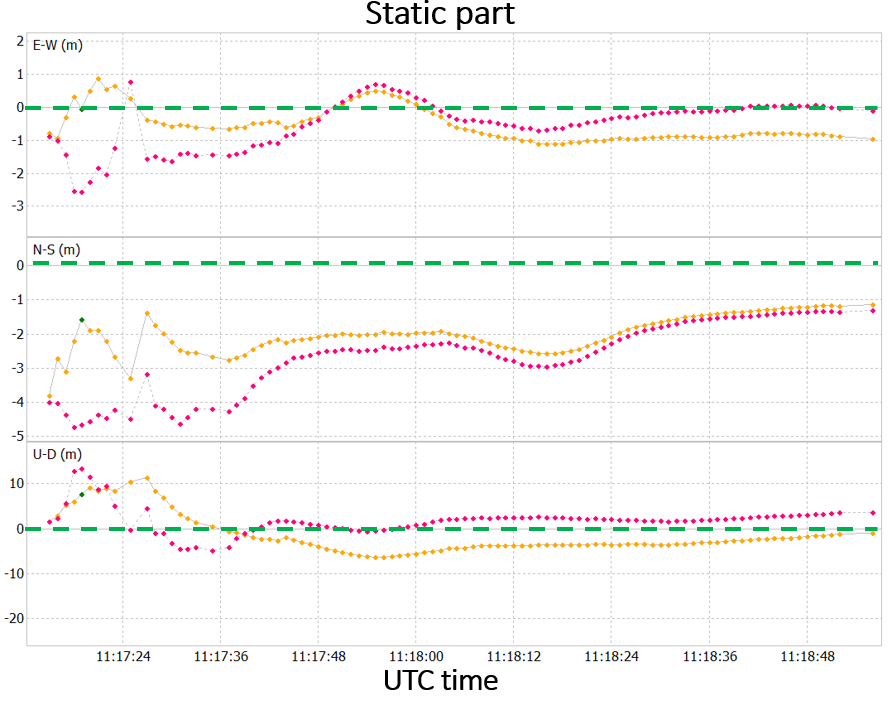
\includegraphics[width=0.48\textwidth]{fig/test3mdp/test3_crit1_mada_static.png}} 
    \subfigure[]{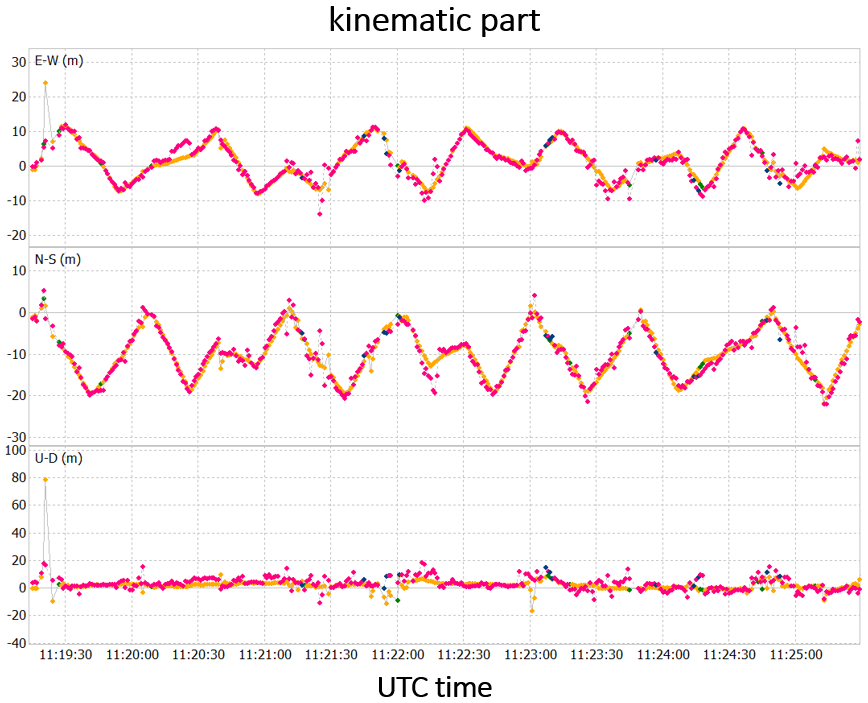
\includegraphics[width=0.48\textwidth]{fig/test3mdp/test3_crit1_mada_kinematic.png}} 
    \caption{Results obtained after the MDP algorithm application using the criterion 1 and adaptive MDP threshold for static part (a) and kinematic part (b)}
    %\label{fig:foobar}
	\label{FIG:test3mdp_crit1mdpadaptive} 
\end{figure}

Differently for the results obtained for the static MDP threshold, the solution accuracy in this case is degraded if the static part of the dataset is considered. The RMS values in fact are increased of about 13 cm and 78 cm for the East and North components, while for 
the Height component an improvement of 92 cm is registered, as shown in Table \ref{tab:test3mpd_crit1_mdp_adaptive}. 

\begin{table}[H]
	\centering
	\begin{tabular}{|p{4.5cm}|c|c|c|c|}
	\hline
	\textbf{Processing} & \textbf{RMS E [m]} & \textbf{RMS N [m]} &
	\textbf{RMS H [m]}&
	\textbf{RMS 2D [m]}\\
    \hline
	No MDP & 0.786 & 1.912 & 3.827&4.340\\  
    \hline
	 MDP, crit 1, adaptive MDP thr & 0.867 & 2.845& 3.521&5.949\\ \hline
	\end{tabular} 
	\caption{RMS obtained for criterion 1, adaptive MDP threshold}
	\label{tab:test3mpd_crit1_mdp_adaptive}
\end{table}

This result highlights that for this case study, the adaptive SNR threshold seems to be less effective in multipath recognition. Nevertheless a significant improvement in the position accuracy can be noted for East and North component after the 11:18 UTC. After this instant the planimetric accuracy is improved of about 11 cm, as the 2D RMS passes from 3.642 m to 3.528 m. This means that the bad performance of the MDP multipath detection are limited to the first few epochs of the dataset. 

Concerning the kinematic part of the dataset a similar behaviour to the one observed for the static MDP threshold is obtained. Nevertheless in this case some improvements are shown. The adaptive MDP threshold solution in fact does not have some outliers that the static MDP solution presents, especially for the Height component (i.e. the ones observed between the 11:21:00 and the 11:21:30 UTC, 11:24:00 and the 11:24:30 UTC cfr Fig. \ref{FIG:test3mdp_crit1mdpstatic}). This means that, if the criterion 1 is considered for kinematic datasets the usage of the adaptive MDP threshold seems preferable to the usage a static MDP threshold.

Hereafter the results for the criterion 2 are exposed with particular attention to the role played by the SNR threshold in the detection part of the MDP algorithm. As previously explained different SNR threshold values together with different MDP static threshold values were tested. Also different SNR threshold values were tested using the adaptive MDP threshold. 
Between all the MDP static threshold values considered, the best results were obtained for threshold value equal to 2.5 m, coherently with the results observed for criterion 1. In the following discussion therefore only this MDP static threshold value is considered. Varying the SNR threshold value it was noted that the solution accuracy, at least for the static part, improves as the threshold value increases. A further processing was carried out by raising the SNR threshold value from 35 to 40 DB-Hz, but no significant differences were noted. The results for the SNR threshold equal to 35 DB-Hz are shown in Figure \ref{FIG:test3mdp_crit2m25s35}.

\begin{figure}[H] 
	\centering
    \subfigure[]{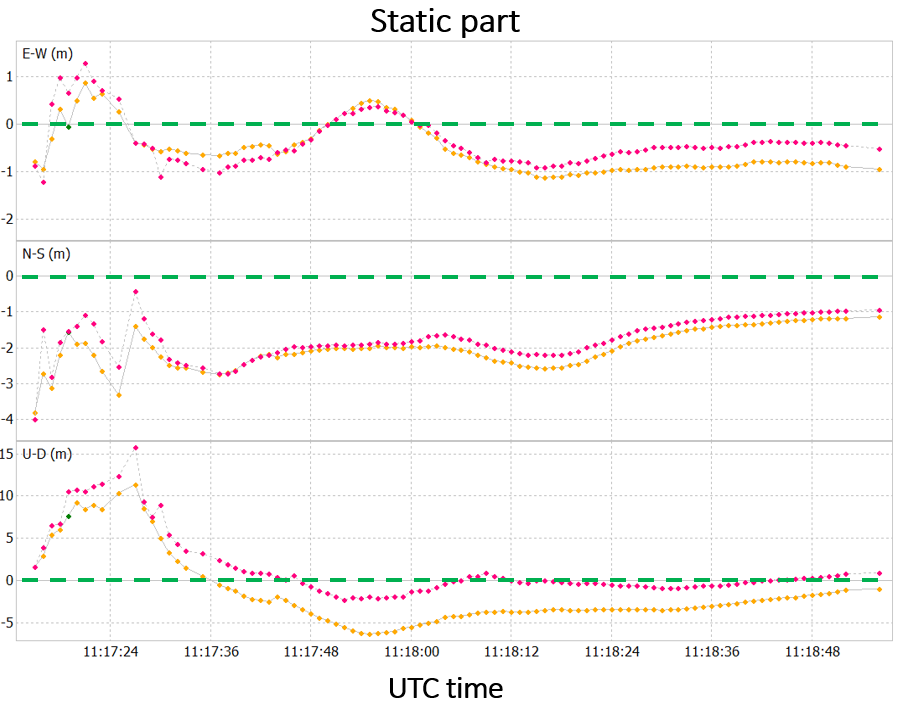
\includegraphics[width=0.48\textwidth]{fig/test3mdp/test3_crit2_m25_s35_static.png}} 
    \subfigure[]{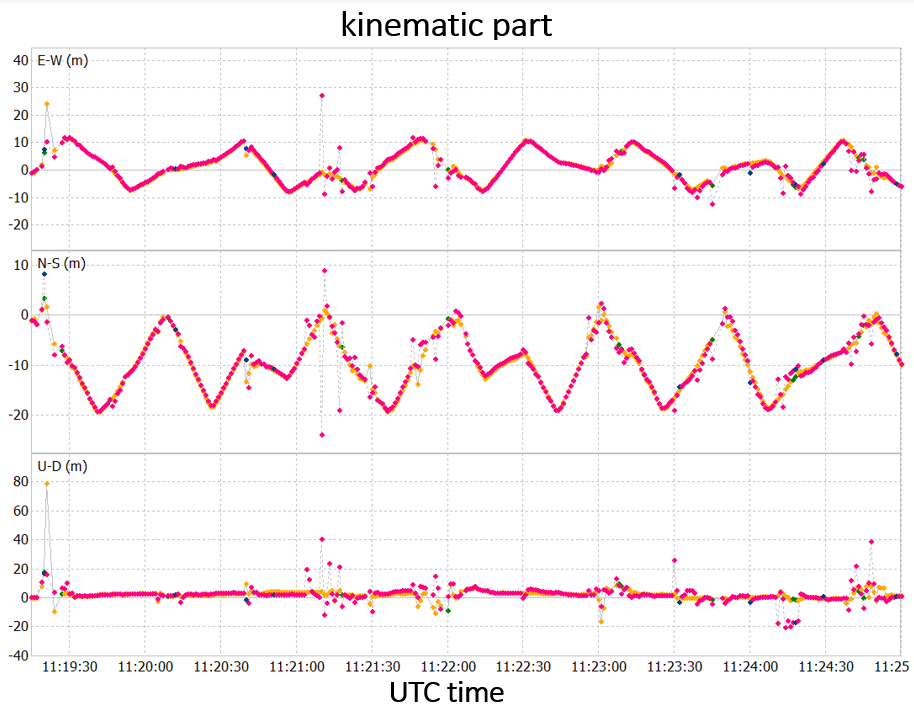
\includegraphics[width=0.48\textwidth]{fig/test3mdp/test3_crit2_m25_s35_kinematic.png}} 
    \caption{Results obtained after the MDP algorithm application using the criterion 2, static MDP threshold = 2.5 m and SNR threshold = 35 DB-Hz, for static part (a) and kinematic part (b)}
   % \label{fig:foobar}
	\label{FIG:test3mdp_crit2m25s35} 
\end{figure}

The statistics in terms of RMS referred to the static part of this solution are exposed in Table \ref{tab:test3mpd_crit2_mdp_static}.

\begin{table}[H]
	\centering
	\begin{tabular}{|p{4.5cm}|c|c|c|c|}
	\hline
	\textbf{Processing} & \textbf{RMS E [m]} & \textbf{RMS N [m]} &
	\textbf{RMS H [m]}&
	\textbf{RMS 2D [m]}\\
    \hline
	No MDP & 0.731 & 2.075& 4.444&4.340\\  
    \hline
	 MDP, crit 2, MDP thr = 2.5 m, SNR thr = 35 DB-Hz& 0.542 &1.722&3.929&3.611\\ \hline
	\end{tabular} 
	\caption{RMS obtained for criterion 2, MDP static threshold}
	\label{tab:test3mpd_crit2_mdp_static}
\end{table}

From the SNR value reported, we observe that the accuracy of the solution in this interval is improved of about 19 cm, 35 cm and 52 cm for the East, North and Height component respectively.The planimetric accuracy of the solution is improved of 73 cm. It's interesting also to notice the difference in RMS between this solution and the one obtained for the criterion 1 (cfr table \ref{tab:test3mpd_crit1_mdp_static}), i.e. without the usage of SNR for the multipath detection part. Considering the planimetric accuracy an improvement of 16 cm is obtained for the criterion 2 case.
Concerning the kinematic part no substantial differences are observed with respect to the criterion 1 case (cfr Fig. \ref{FIG:test3mdp_crit2m25s35}b and Fig. \ref{FIG:test3mdp_crit1mdpstatic}b). 
It can be stated then that the solution obtained for the criterion 2 is better in terms of accuracy with respect to the one obtained for the criterion 1, in case of an MDP static threshold, especially for the static part of the test. So in static condition, considering both the SNR and MDP values for the detection part of the MDP algorithm increases the performance of the algorithm itself. The situation is different for the kinematic part, in which no differences are noted. In this case it seems that using the SNR value does not take any advantage to the detection part of the MDP algorithm.

The test  with criterion 2 also involved  the usage of the adaptive MDP threshold. In this cases, varying the SNR threshold value, no significant differences were reported to the results already obtained for the criterion 1 so the results are not shown. It can be state then that, for criterion 2, if the adaptive MDP threshold is considered, the usage of the SNR value does not improve the performance of the detection part of the MDP algorithm.

Lastly the criterion 3 is considered for the processing referred to this dataset. Considering the static MDP threshold, coherently to the results obtained for the others two criteria, the major improvements are obtained for MDP threshold equal to 2.5 m, so the impact of the SNR value is discussed only for this situation.  In criterion 3, improvements in the solution are observed only for SNR values lower than 30 DB-Hz, and the best results are obtained for SNR threshold equal to 25 DB-Hz. Fig. \ref{FIG:test3mdp_crit3m25s25} shows the results obtained for this case.

\begin{figure}[H] 
	\centering
    \subfigure[]{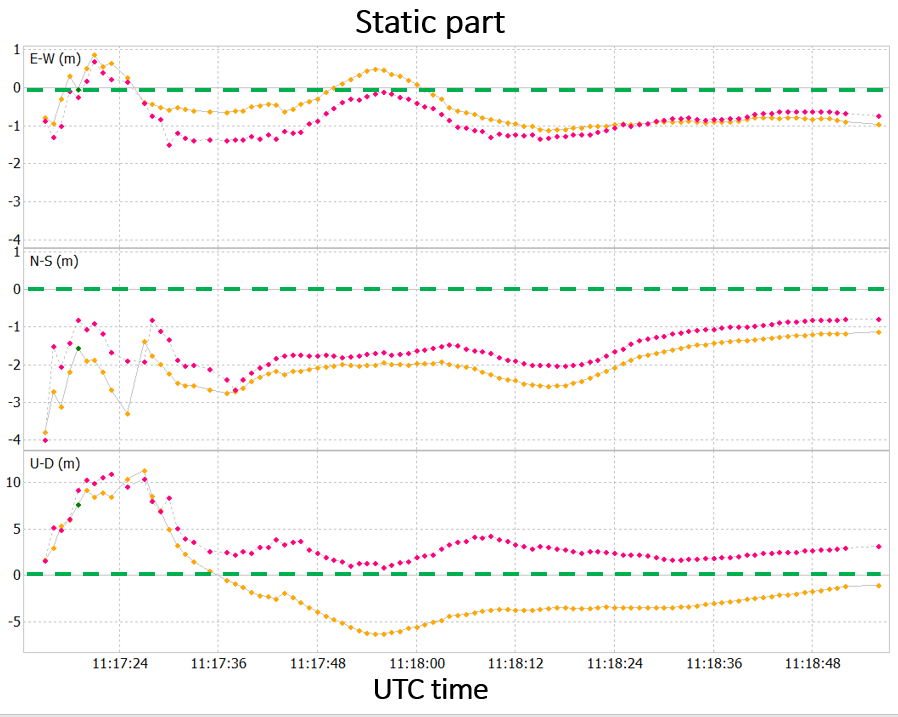
\includegraphics[width=0.48\textwidth]{fig/test3mdp/test3_crit3_m25_s25_static.png}} 
    \subfigure[]{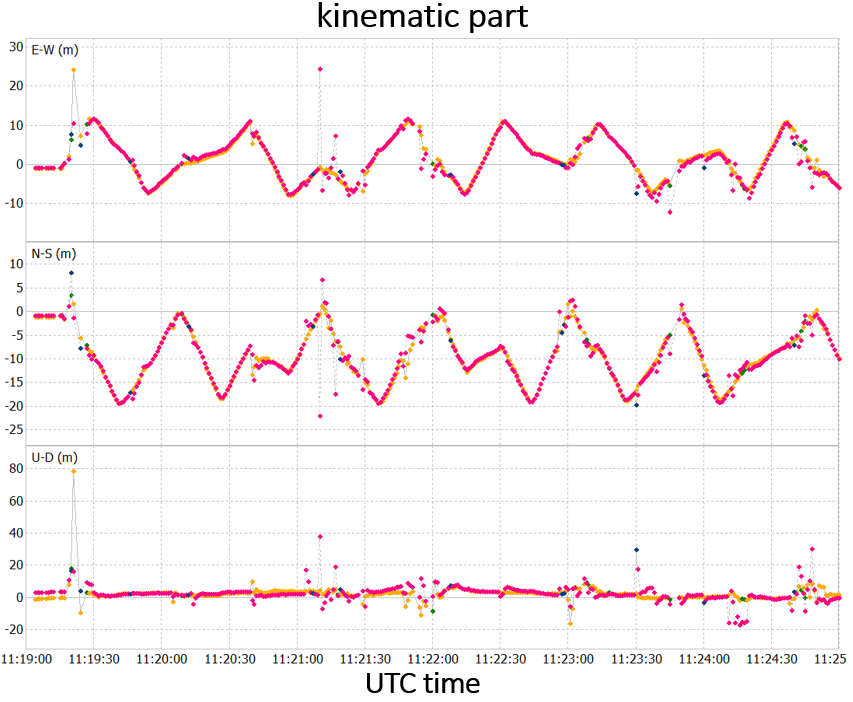
\includegraphics[width=0.48\textwidth]{fig/test3mdp/test3_crit3_m25_s25_kinematic.png}} 
    \caption{Results obtained after the MDP algorithm application using the criterion 3, static MDP threshold = 2.5 m and SNR threshold = 25 DB-Hz, for static part (a) and kinematic part (b)}
    %\label{fig:foobar}
	\label{FIG:test3mdp_crit3m25s25} 
\end{figure}

The RMS for the static part are reported in Table \ref{tab:test3mpd_crit3_mdp_static}. With the aim of highlighting the worsening of the solution accuracy as the SNR threshold value increases, also the statistics related to the case having SNR threshold equal to 35 DB-Hz are reported in the table.

\begin{table}[H]
	\centering
	\begin{tabular}{|p{4.5cm}|c|c|c|c|}
	\hline
	\textbf{Processing} & \textbf{RMS E [m]} & \textbf{RMS N [m]} &
	\textbf{RMS H [m]}&
	\textbf{RMS 2D [m]}\\
    \hline
	No MDP & 0.731 & 2.075& 4.444&4.340\\  
    \hline
	 MDP, crit 3, MDP thr = 2.5 m, SNR thr = 25 DB-Hz& 0.935 &1.638&4.063&3.772\\ \hline
	 MDP, crit 3, MDP thr = 2.5 m, SNR thr = 35 DB-Hz&1.234 &3.412&2.824&7.256\\ \hline
	\end{tabular} 
	\caption{RMS obtained for criterion 3, MDP static threshold}
	\label{tab:test3mpd_crit3_mdp_static}
\end{table}

The values in Table \ref{tab:test3mpd_crit3_mdp_static} show that if the SNR threshold equal to 25 DB-Hz is considered, the RMS is increased for North and Height component, while it is deteriorated for the East component. Nevertheless, the planimetric accuracy for this case in improved of about 57 cm. 
Concerning the case having the SNR threshold equal to 35 DB-Hz it's evident that the overall solution accuracy id degraded, as the RMS of all the components presents higher values with respect to the ``No MDP" case. This results confirms what has already been observed for the previous case study, i.e., using the MDP algorithm with high SNR threshold in the criterion 3 leads to a degraded solution. Indeed, 
in this case too many observables are wrongly identified as multipath affected and consequently underweighted.

The kinematic part of this dataset shows an analog behaviour to the one obtained for the processing carried out for the criteria 1 and 2 (cfr Figures \ref{FIG:test3mdp_crit1mdpstatic}b and \ref{FIG:test3mdp_crit2m25s35}b). No further improvements are observed for this case study and the same considerations, already discussed for the other cases, are valid also for this obtained result. 

Similar considerations can be also retrieved if the adaptive MDP threshold is adopted in the criterion 3. In this case, if an SNR threshold lower than 25 DB-Hz no significant differences were reported to the results already obtained for the criterion 1 (cfr figure \ref{FIG:test3mdp_crit1mdpadaptive} and table \ref{tab:test3mpd_crit1_mdp_adaptive}). Problems arise when SNR threshold values higher than 30 DB-Hz are considered. As a matter of example, if the SNR threshold value is set to 35 DB-Hz (worst result obtained), during the initial static part of the dataset the planimetric accuracy of the obtained solution is degraded of about 3.5 m with respect to the ``No MDP" case (7.888 m against 4.340 m). This result confirms that if high value of SNR threshold are used in the criterion 3 the multipath detection capability of the MDP algorithm is compromised and coarser results are obtained with respect to the ones retrieved without the application of the algorithm. 

%(da qui in poi non so se lasciare qua o spostare nelle conclusioni)


%In this chapter, the performance of the solution proposed to improve the accuracy in the GNSS positioning from Android devices has been tested. This solution is based on an architecture which enables the RTK positioning for Android devices and on the application of MDP algorithm for the multipath detection and mitigation. For this purpose both static dataset with multipath induced, and kinematic dataset were analysed and discussed. The MDP algorithm showed promising results in multipath detection and mitigation, especially in static condition. From the static dataset, it comes clear in fact that the solution accuracy is improved for all the tested configurations. Furthermore, the higher improvements were observed during the multipath induced interval, confirming the algorithm capability to recognise and mitigate this effect. The algorithm not only increases the accuracy, but also eliminates some false fixed positions, increasing then the solution robustness.
%Nevertheless, the MDP algorithm detection capabilities need to be studied in deeper detail, especially for Android GNSS receivers that 
 %present very noisy observables. Regarding this topic, in this work both a static and adaptive MDP threshold were tested. Concerning the static MDP threshold it was observed that the performance of the algorithm improves as the threshold value decreases. The optimal threshold value found, for both the datasets is 2.5m. Being the multipath effect identified by outliers in the MDP trend (figure \ref{FIG:test4mdp_mdpxiaomiublox}a and \ref{FIG:test3mdp_mdpxiaomistonex}a) and also considering the high noise of smartphone's GNSS observables, which makes the MDP variable higher in modulus, the observables having MDP values lower than 2.5 m can not be considered affected by multipath. The adaptive MDP threshold was also tested showing interesting results. In this case each observable has its own threshold value, and multipath identification seems to be more effective.
 
 %Lastly the effect of SNR were tested for the detection part of the MDP algorithm combining SNR and MDP thresholds by means of two different strategies, i.e. criterion 2 and 3. In criterion 2, the usage of SNR brings benefits to the detection capabilities of the algorithm. The solution accuracy and robustness are increased, especially when high value of SNR threshold (i.e. 35 DB-Hz) are considered. In criterion 3, usage of SNR brings benefits to the detection capabilities of the algorithm only when low SNR threshold are considered (i.e. $<$ 30 DB-Hz). If high SNR threshold are considered in this case, many observables are considered affected by multipath even if they are not. This compromise not only the detection, but also the mitigation performance of the MDP algorithm. For this reason, dealing with very noisy GNSS observables, such as the smartphone's ones, the criterion 3 shouldn't be considered.